\documentclass{esg8012pset}
\begin{preamble}
  \usepackage{amsmath}
  \usepackage{amssymb}
  \usepackage{amsthm}
  \usepackage{enumerate}
  \usepackage{graphicx}
  \usepackage{hyperref}
  %\usepackage{siunitx}
  \providecommand{\uvec}[1]{{\hat{\bf{#1}}}}
  \usepackage{pgf,tikz}
  \usetikzlibrary{arrows}
  \usepackage{wasysym}
  \makeatletter
  \newcommand{\interitemtext}[1]{%
    \begin{list}{}
     {\itemindent=0mm\labelsep=0mm
     \labelwidth=0mm\leftmargin=0mm
     \addtolength{\leftmargin}{-\@totalleftmargin}}
      \item #1
    \end{list}
  }
  \makeatother
  \renewcommand{\d}{\,d}
  \providecommand{\norm}[1]{\lVert#1\rVert}
  \newtheorem{thm}{Theorem}[section]
  \newtheorem*{thm*}{Theorem}
\end{preamble}

\classname{Physics 8.012}
\semester{Fall 2010}
\problemsetnumber{9}
\makeatletter
\duedate{Monday, November 22}
\readingassignment{Kleppner and Kolenkow, \emph{An Introduction to Mechanics}, Chapter Six}

\begin{document}

\noindent Problems: Chapter 6: 14, 18, 24, 29, 30, 37, 41



\begin{problem}{K\&K 6.14}
  A uniform stick of mass $m$ and length $l$ is suspended horizontally with end $B$ at the edge of a table and the other end $A$ is held by hand. Point A is suddenly released. At the instant after release:
  \begin{center}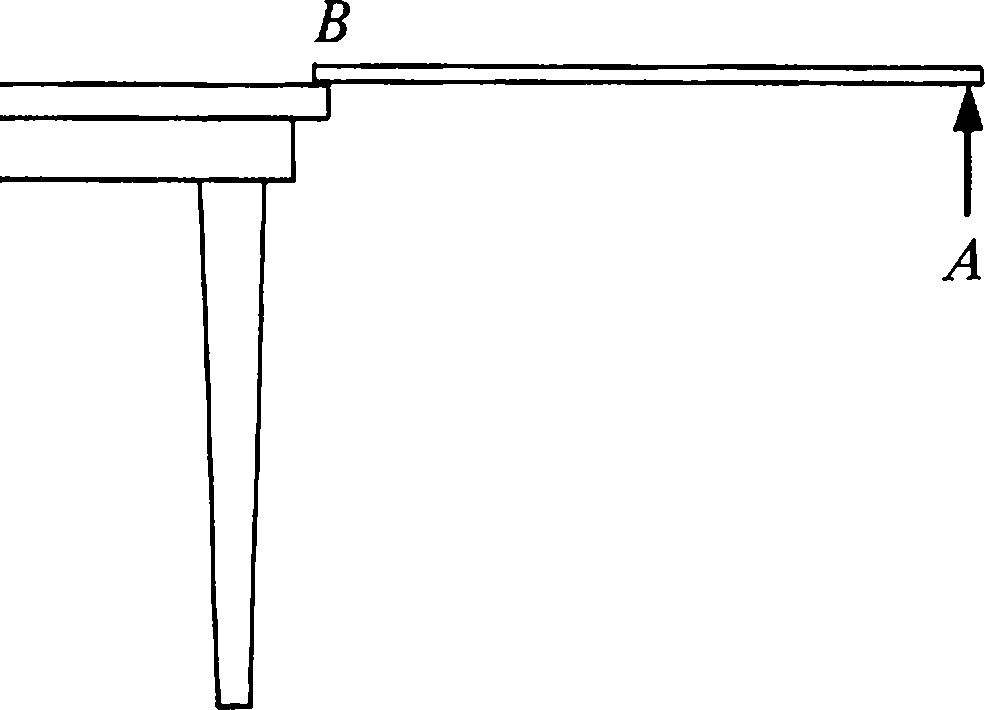
\includegraphics[width=0.33\textwidth]{ps09_1}\end{center}
  \begin{enumerate}[(a)]
    \item What is the torque about the end $B$ on the table?
    \item What is the angular acceleration about the end $B$ on the table?
    \item What is the vertical acceleration of the center of mass?
    \item What is the vertical component of the hinge force at $B$? Does the hinge force have a horizontal component at the instant after release?
  \end{enumerate}
\end{problem}
\begin{solution}
  \begin{enumerate}[(a)]
    \item The center of mass is at a distance $l / 2$ from the table, and so the torque, treating it as a point mass, is $m g l / 2$.  Alternatively, $\vec \tau = \int_0^l \lambda(x) g x \d x = \frac{\lambda l^2 g}{2} = m l g / 2$.
    \item The angular acceleration is \begin{align*}
      \frac{m l g / 2}{\int_0^l \lambda r^2 \d r} & = \frac{m l g / 2}{\frac{m}{l} \int_0^l r^2 \d r } \\
      & = \frac{m l g / 2}{\frac{m}{l} \int_0^l r^2 \d r } \\
      & = \frac{m l g / 2}{\frac{m}{l} \cdot \frac{l^3}{3} } \\
      & = \frac{m l g / 2}{m \frac{l^2}{3} } \\
      & = \frac{g / 2}{\frac{l}{3} } \\
      & = \frac{3 g}{2 l}
      \end{align*}
    \item The vertical acceleration is $r\alpha = \frac{3 g l}{4 l} = \frac{3}{4}g$.
    \item The vertical component of the hinge force is $m\frac{g}{4}$.  The hinge force has no horizontal component, because the center of mass is not accelerating in the horizontal direction.
  \end{enumerate}
\end{solution}





\begin{problem}{K\&K 6.18}
  A physical pendulum consists of a disc of radius $R$ and mass $m_d$ fixed at the end of a rod of mass $m_r$ and length $l$.
  \begin{center}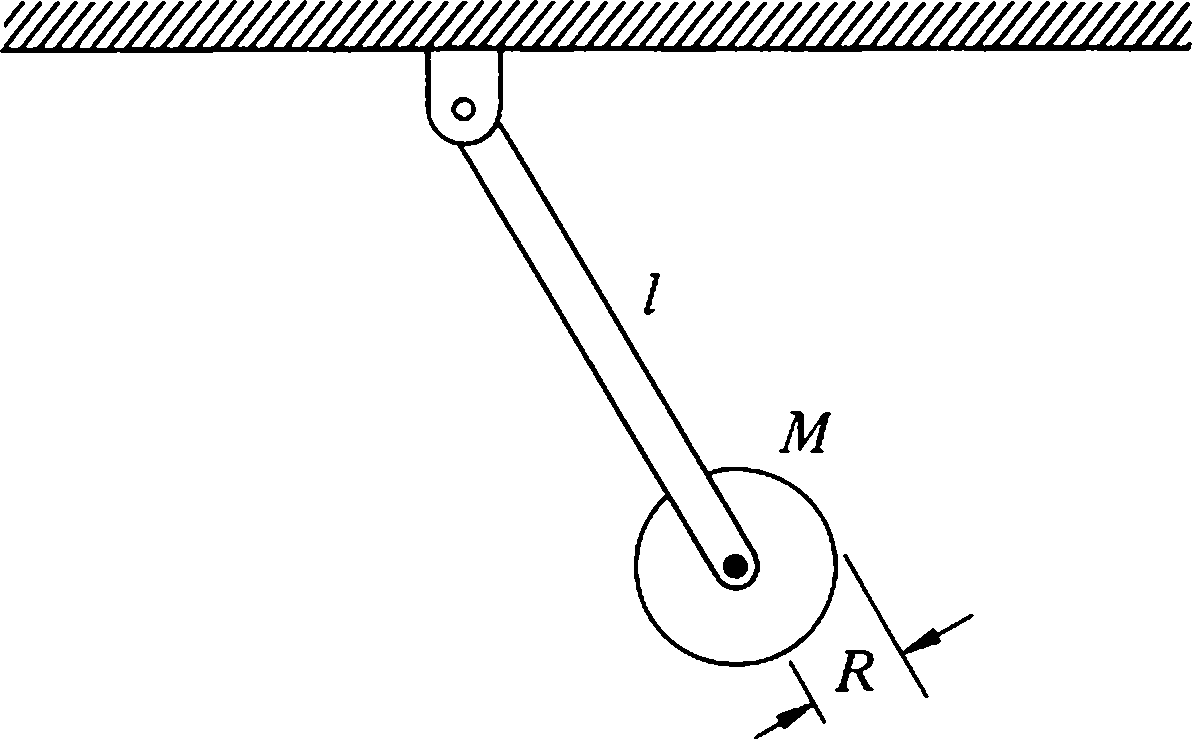
\includegraphics[width=0.3\textwidth]{ps09_2}\end{center}
  \begin{enumerate}[(a)]
    \item Find the period of the pendulum.
    \item How does the period change if the disk is mounted to the rod by a frictionless bearing so that it is perfectly free to spin?
  \end{enumerate}
\end{problem}
\begin{solution}
  \begin{enumerate}[(a)]
    \item Since the pendulum is a rigid body, and the the center of mass is at length $\frac{m_d l + m_r l / 2}{m_d + m_r}$, the forces can be taken to act at this point.  Let $\theta$ be the angle from the vertical.  Then $\tau = \frac{m_d l + m_r l / 2}{m_d + m_r} (m_d + m_r)g\sin\theta = (m_d l + m_r l / 2)g\sin\theta$.  Then $\frac{\d L}{\d t} = (m_d l + m_r l / 2)g\sin\theta$.
    \begin{thm}[Parallel Axis Theorem]
    Suppose $\ell_1$ and $\ell_2$ are parallel axes, and $\ell_1$ is through the center of mass, and $\vec d = d\hat d$ is the vector from $\ell_2$ and $\ell_1$.  Suppose that $s$ is a point on $\ell_1$ and $s' = s + \vec d$ is a point on $\ell_2$.  Then, for any rigid object of total mass $m_T$, rotating about the fixed axis $\ell_2$, \begin{equation} I_{\ell_1} + m_T d^2 = I_{\ell_2} \end{equation}
    \end{thm}
    \begin{proof}
      \begin{align*}
        (\vec L_{s'})_{\ell_2} & = \sum_i (\vec r_{s'i} \times m_i\vec v_i)_{\ell_2} \\
        & = \sum_i (\vec r_{s'i} \times m_i(\vec \omega_i \times \vec r_{s'i}))_{\ell_2} \\
        & = \sum_i (\vec r_{s'i} \times m_i(\omega_i r_{\ell_2 i} \hat v))_{\ell_2} \\
  \intertext{We may discard the non-vertical components because we are concerned only with the angular momentum about $\ell_1$.  Then}
        (\vec L_{s'})_{\ell_2} & = \sum_i \vec r_{\ell_2 i} \times m_i(\omega_i r_{\ell_2 i} \hat v) \\
        & = \vec \omega \sum_i \vec r_{\ell_2 i}^2 m_i \\
        & = \vec \omega I_{\ell_2} \\
        & = \vec \omega \sum_i r_{\ell_2 i}^2 m_i \\
        & = \vec \omega \sum_i (\vec d + r_{\ell_1 i})^2 m_i \\
        & = \vec \omega \sum_i (d^2 + r_{\ell_1 i}^2 + 2\vec d \cdot \vec r_{\ell_1 i}) m_i \\
        & = \vec \omega \left( d^2 \sum_i m_i +  \sum_i r_{\ell_1 i}^2 m_i + 2\vec d \cdot \sum_i \vec r_{\ell_1 i} m_i \right) \\
        & = \vec \omega \left( d^2 m_T +  I_{\ell_1} + 2\vec d \cdot \vec 0 \right) \\
        & = \vec \omega \left( d^2 m_T +  I_{\ell_1} \right) \\
        \\
        I_{\ell_2} & = I_{\ell_1} + d^2 m_T
      \end{align*}
    \end{proof}
    $\alpha = \ddot\theta = \frac{\d L / \d t}{I}$.  \begin{align*}
    I & = m_r\int_0^l r^2 \d r + m_d l^2 + \int_0^R \frac{m_d 2 \pi r}{\pi R^2} r^2 \d r \\
      & = m_r\frac{l^3}{3} + m_d l^2 + \frac{m_d 2}{R^2}\int_0^R r^3 \d r \\
      & = m_r\frac{l^3}{3} + m_d l^2 + \frac{m_d 2 R^4}{4 R^2} \\
      & = m_r\frac{l^3}{3} + m_d l^2 + \frac{m_d R^2}{2}
    \end{align*} Then $\ddot \theta = \frac{-(m_d l + m_r l / 2)g\sin\theta}{m_r\frac{l^3}{3} + m_d l^2 + \frac{m_d R^2}{2}}$.  Using the small angle approximation of $\sin\theta\approx \theta$, $\frac{\d^2 \theta}{\d t^2} = -\frac{(m_d l + m_r l / 2)g}{m_r\frac{l^3}{3} + m_d l^2 + \frac{m_d R^2}{2}}\theta$.  Then $\omega = \sqrt{\frac{(m_d l + m_r l / 2)g}{m_r\frac{l^3}{3} + m_d l^2 + \frac{m_d R^2}{2}}}$ and the period is $\frac{2\pi}{\sqrt{\frac{(m_d l + m_r l / 2)g}{m_r\frac{l^3}{3} + m_d l^2 + \frac{m_d R^2}{2}}}}$.
    \item If the disc is allowed to rotate freely, then the disc acts as a point mass on the end of the rod.  Then $I = m_r\frac{l^3}{3} + m_d l^2$, so $\ddot \theta = \frac{-(m_d l + m_r l / 2)g\sin\theta}{m_r\frac{l^3}{3} + m_d l^2}$.  Using the small angle approximation of $\sin\theta\approx \theta$, $\frac{\d^2 \theta}{\d t^2} = -\frac{(m_d l + m_r l / 2)g}{m_r\frac{l^3}{3} + m_d l^2}\theta$.  Then $\omega = \sqrt{\frac{(m_d l + m_r l / 2)g}{m_r\frac{l^3}{3} + m_d l^2}}$ and the period is $\frac{2\pi}{\sqrt{\frac{(m_d l + m_r l / 2)g}{m_r\frac{l^3}{3} + m_d l^2}}}$.
  \end{enumerate}
\end{solution}





\begin{problem}{K\&K 6.24}
  A drum $A$ of mass $m$ and radius $R$ is suspended from a drum $B$ also of mass $m$ and radius $R$, which is free to rotate about its axis. The suspension is in the form of a massless metal tape wound around the outside of each drum, and free to unwind. Gravity is directed downwards. Both drums are initially at rest. Find the initial acceleration of drum $A$, assuming that it moves straight down.
  \begin{center}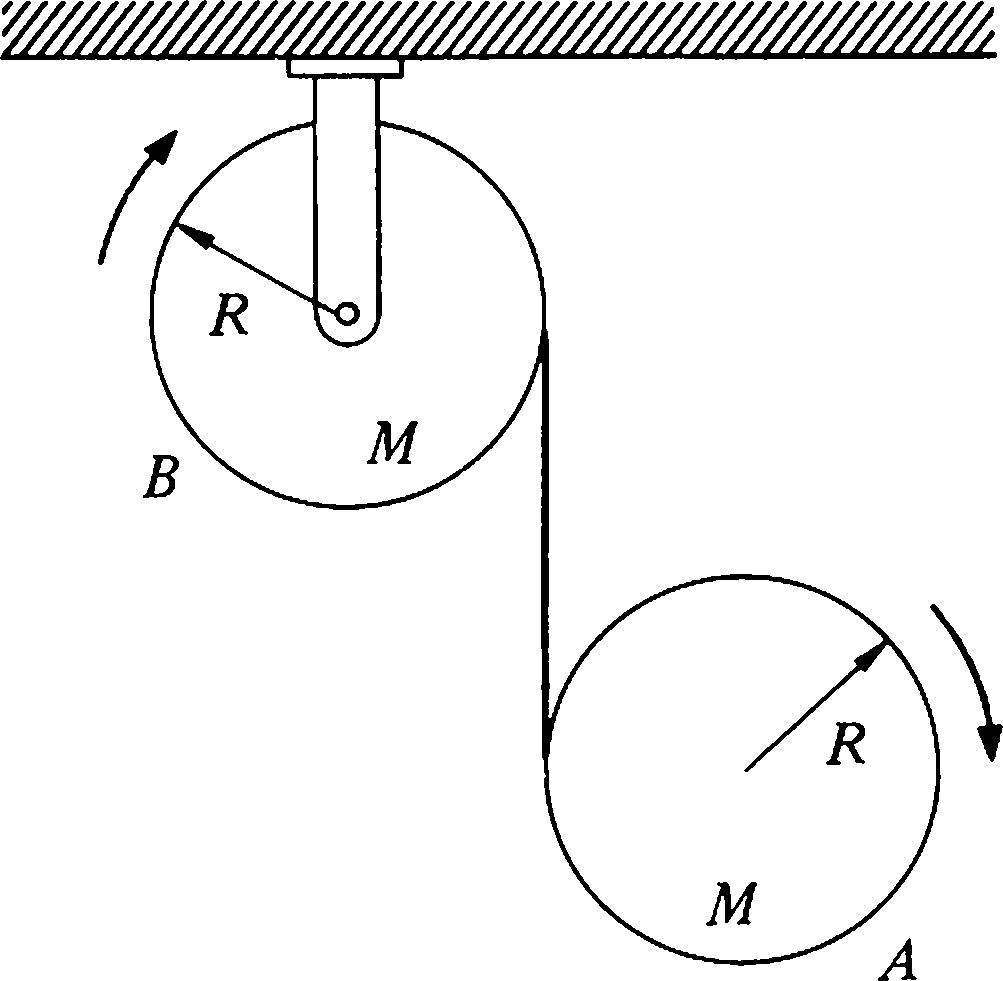
\includegraphics[width=0.25\textwidth]{ps09_3}\end{center}
\end{problem}
\begin{solution}
  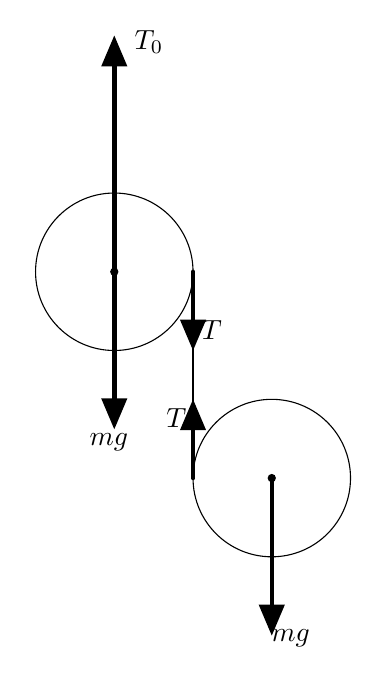
\begin{tikzpicture}[line cap=round,line join=round,>=triangle 45,x=1.0cm,y=1.0cm]
  \clip(-1.1,0) rectangle (3.1,8.1);
  \draw(0,5) circle (1cm);
  \draw(2,2.38) circle (1cm);
  \draw (1,5)-- (1,2.38);
  \draw [->,line width=1.6pt] (1,5) -- (1,4);
  \draw [->,line width=1.6pt] (1,2.38) -- (1,3.38);
  \draw [->,line width=1.6pt] (0,5) -- (0,3);
  \draw [->,line width=1.6pt] (2,2.38) -- (2,0.38);
  \draw [->,line width=1.6pt] (0,5) -- (0,8);
  \fill [color=black] (0,5) circle (1.5pt);
  \fill [color=black] (2,2.38) circle (1.5pt);
  \draw[color=black] (1.24,4.26) node {$T$};
  \draw[color=black] (0.79,3.14) node {$T$};
  \draw[color=black] (-0.07,2.84) node {$m g$};
  \draw[color=black] (2.24,0.35) node {$m g$};
  \draw[color=black] (0.44,7.92) node {$T_0$};
  \end{tikzpicture}

  Since the tape is massless and rigid, the tension on $A$ is the same as the tension on $B$.  Let $\ell$ be the length of the tape.  Then $\frac{\d \ell}{\d t} = \omega_B R + \omega_A R = v_A$.  Then $\ddot \ell = R (\alpha_A + \alpha_B) = a_A = g - \frac{T}{m}$.  Since $\vec \tau = \vec r \times \vec F$, and $I_{\text{disc}} = \int_0^R r^2 \frac{2\pi r m_T}{\pi R^2} \d r = \frac{2 m_T}{R^2} \cdot \frac{R^4}{4} = \frac{m_T R^2}{2}$, \begin{align*}
  R (\alpha_A + \alpha_B) & = g - \frac{T}{m} \\
  R \frac{\tau_A + \tau_B}{m R^2 / 2} & = g - \frac{T}{m} \\
  2\cdot \frac{\tau_A + \tau_B}{m R} & = g - \frac{T}{m} \\
  2\cdot \frac{T R + T R}{m R} & = g - \frac{T}{m} \\
  \frac{4T}{m} & = g - \frac{T}{m} \\
  T & = \frac{1}{5}m g
  \end{align*}  Then $a_A = \frac{4}{5}g$.
\end{solution}





\begin{problem}{K\&K 6.29}
  A Yo-Yo of mass $m$ has an axle of radius $b$ and a spool of radius $R$. It's moment of inertia can be taken to be $I = (1/2)mR^2$ and the thickness of the string can be neglected.

  The Yo-Yo is released from rest.
  \begin{center}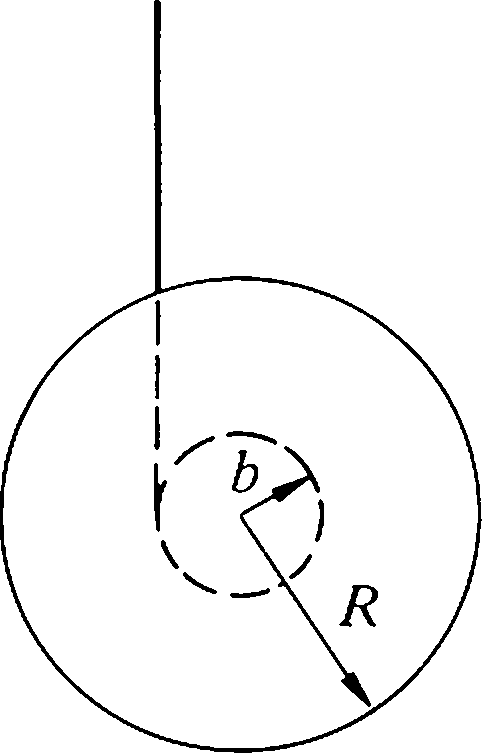
\includegraphics[width=0.15\textwidth]{ps09_4}\end{center}
  \begin{enumerate}[(a)]
    \item What is the tension in the cord as the Yo-Yo descends and as it ascends?
    \item The center of the Yo-Yo descends a distance $h$ before the string is fully unwound. Use conservation of energy to find the angular velocity of the Yo-Yo when it reaches its lowest point.
    \item What happens to the Yo-Yo at the bottom of the string?
    \item Assuming it reverses direction with uniform angular velocity, find the average force on the string while the Yo-Yo turns around.
  \end{enumerate}
\end{problem}
\begin{solution}
  \begin{enumerate}[(a)]
    \item Let $y$ be the position of the Yo-Yo, with the up direction and clockwise direction positive, and let $\ell$ be the length of the string which is unwound.  Then $\frac{\d y}{\d t} = -\frac{\d \ell}{\d t} = -\omega b$.  Since $\ddot y = - g + \frac{T}{m} = -\alpha b$ and $\alpha = \frac{\tau}{I} = \frac{T b}{m R^2 / 2}$, $- g + \frac{T}{m} = -\frac{T b^2}{m R^2 / 2}$.  Then $m g = T\left(1 + \frac{2b^2}{R^2}\right)$, so $T = \frac{m g}{1 + \frac{2b^2}{R^2}} = \frac{m g R^2}{R^2 + 2b^2}$. \par
      Going up, $\frac{\d y}{\d t} = -\frac{\d \ell}{\d t} = \omega b$.  Since $\ddot y = -g + \frac{T}{m} = \alpha b$ and $\alpha = \frac{\tau}{I} = \frac{T b}{m R^2 / 2}$, $- g + \frac{T}{m} = \frac{T b^2}{m R^2 / 2}$.  Then $m g = T\left(1 - \frac{2b^2}{R^2}\right)$, so $T = \frac{m g}{1 - \frac{2b^2}{R^2}} = \frac{m g R^2}{R^2 - 2b^2}$.
    \item Since $\omega_f b = v_f$.  Then $m g h = \frac{1}{2} m v_f^2 + \frac{1}{2} I \omega_f^2 = \frac{1}{2} m b^2 \omega_f^2 + \frac{1}{4}mR^2 \omega_f^2$.  Then $\omega_f = \sqrt{\frac{2 g h}{b^2+R^2/2}}$.
    \item Assuming there is a fixed point, the Yo-Yo rotates about its point of contact with the string.  (FIX)
    \item Assuming that the speed remains constant, the average tension is $\frac{1}{\pi}\int_0^\pi \frac{m v_f^2}{R} + \sin\theta m g = \frac{m v_f^2}{b} + 2 m g$.
  \end{enumerate}
\end{solution}




\clearpage
\begin{problem}{K\&K 6.30}
  A bowling ball of mass $m$ and radius $R$ is initially thrown down an alley with an initial velocity $v_0$ and it slides without rolling but due to friction it begins to roll. The moment of inertia of the ball about its center of mass is $I_\text{cm} = (2/5) mR^2$. What is the velocity of the bowling ball when its just start to roll without slipping.
  \begin{center}
    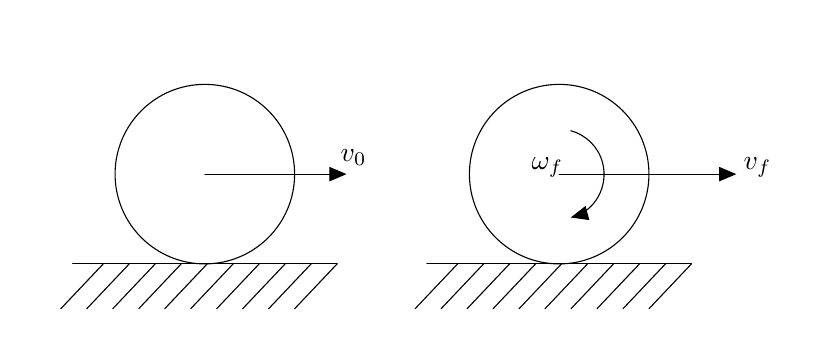
\begin{tikzpicture}[line cap=round,line join=round,>=triangle 45,x=3.0cm,y=3.0cm]
    \clip(-1.5,-0.25) rectangle (1.75,1);
    \draw(0.75,0.38) circle (0.38);
    \draw(-0.75,0.38) circle (0.38);
    \draw [->] (-0.75,0.38) -- (-0.15,0.38);
    \draw [->] (0.75,0.38) -- (1.5,0.38);
    %\draw [shift={(-0.75,0.38)},->] (-75:0.19) arc (75:0.19);
    %\draw [shift={(-0.75,0.38)},color=black,<-] (-75:0.19) arc (-75:75:0.19);
    \draw [shift={(0.75,0.38)},color=black,<-] (-75:0.19) arc (-75:75:0.19);
    %\draw [shift={(-0.75,0.38)}] plot[domain=-1.18:1.18,variable=\t]({1*0.19*cos(\t r)+0*0.19*sin(\t r)},{0*0.19*cos(\t r)+1*0.19*sin(\t r)});
    %\draw [shift={(0.75,0.38)}] plot[domain=-1.18:1.18,variable=\t]({1*0.19*cos(\t r)+0*0.19*sin(\t r)},{0*0.19*cos(\t r)+1*0.19*sin(\t r)});
    \draw (-1.31,0)-- (-0.19,0);
    \draw (0.19,0)-- (1.31,0);
    \draw (-0.19,0)-- (-0.37,-0.19);
    \draw (1.31,0)-- (1.13,-0.19);
    \draw (-0.3,0)-- (-0.48,-0.19);
    \draw (-0.41,0)-- (-0.59,-0.19);
    \draw (-0.52,0)-- (-0.7,-0.19);
    \draw (-0.63,0)-- (-0.81,-0.19);
    \draw (-0.74,0)-- (-0.92,-0.19);
    \draw (-0.85,0)-- (-1.03,-0.19);
    \draw (-0.96,0)-- (-1.14,-0.19);
    \draw (-1.07,0)-- (-1.25,-0.19);
    \draw (-1.18,0)-- (-1.36,-0.19);
    \draw (1.2,0)-- (1.02,-0.19);
    \draw (1.09,0)-- (0.91,-0.19);
    \draw (0.98,0)-- (0.8,-0.19);
    \draw (0.87,0)-- (0.69,-0.19);
    \draw (0.76,0)-- (0.58,-0.19);
    \draw (0.65,0)-- (0.47,-0.19);
    \draw (0.54,0)-- (0.36,-0.19);
    \draw (0.43,0)-- (0.25,-0.19);
    \draw (0.32,0)-- (0.14,-0.19);
    \draw[color=black] (-0.12,0.45) node {$v_0$};
    \draw[color=black] (1.59,0.41) node {$v_f$};
    %\draw[color=black] (-0.85,0.41) node {$\omega_0$};
    \draw[color=black] (0.7,0.41) node {$\omega_f$};
    \end{tikzpicture}
  \end{center}
\end{problem}
\begin{solution}
The final angular velocity is such that $\omega_f R = v_f$.  The force of friction is such that $m \dot v = F_{fr}$ and $R\times F_{fr} = I\dot\omega$.  Then \begin{align*}
\int_0^{t_f} m \dot v \d t & = \int_0^{t_f} \frac{I}{R} \dot\omega \d t \\
m(v_f - v_0) & = \frac{I}{R}(\omega_f - \omega_0) \\
m(v_f - v_0) & = \frac{I}{R}\omega_f \\
m(v_f - v_0) & = \frac{I v_f}{R^2}\\
v_f & = \frac{I v_f}{m R^2} + v_0
\end{align*}
\end{solution}




\begin{problem}{K\&K 6.37}
  A hockey puck of mass $m_1$ slides along ice with a velocity $v_0$ and strikes one end of a stick lying on the ice of length $l_2$ and mass $m_2$. The center of mass of the stick moves with an unknown magnitude $v_{cm}$. The stick also rotates about the center of mass with unknown angular velocity $\omega_{f}$. The puck continues to move in the same straight line as before it hit the stick with velocity $v_f$. Assume the ice is frictionless and there is no loss of mechanical energy during the collision.
  \begin{center}
    \begin{tikzpicture}[line cap=round,line join=round,>=triangle 45,x=2.0cm,y=2.0cm]
    \clip(-2,-1.5) rectangle (2.5,1.75);
    \draw [shift={(1.4,0)},->] (-75:0.5) arc (-75:75:0.5);
    \draw [->] (0,0.33) -- (0,1);
    \draw [->] (0,-0.33) -- (0,-1);
    \draw (-0.1,0.19) node[anchor=north west] {$\ell_2$};
    \draw (-1.1,1)-- (-0.9,1);
    \draw (-0.9,1)-- (-0.9,-1);
    \draw (-0.9,-1)-- (-1.1,-1);
    \draw (-1.1,-1)-- (-1.1,1);
    \draw (0.9,1)-- (1.1,1);
    \draw (1.1,1)-- (1.1,-1);
    \draw (1.1,-1)-- (0.9,-1);
    \draw (0.9,-1)-- (0.9,1);
    \draw(-1.77,-1) circle (0.1cm);
    \draw(1.77,-1) circle (0.1cm);
    \draw [->] (-1.65,-1) -- (-1.35,-1);
    \draw [->] (1.89,-1) -- (2.19,-1);
    \draw [->] (1,0) -- (1.4,0);
    \draw (-1.1,0.17) node[anchor=north west] {$x$};
    \draw[color=black] (-1.76,-1.15) node {$m_1$};
    \draw[color=black] (1.79,-1.17) node {$m_1$};
    \draw[color=black] (-1.25,-1) node {$v_0$};
    \draw[color=black] (2.3,-1) node {$v_f$};
    \draw[color=black] (1.63,0) node {$v_\text{cm}$};
    \draw[color=black] (2.09,0) node {$\omega_f$};
    \draw (-1.5,1.05) node[anchor=north west] {$m_{2}$};
    \end{tikzpicture}
  \end{center}
  \begin{enumerate}[(a)]
    \item Write down the equation for conservation of momentum.
    \item Write down the equation for conservation of energy.
    \item Is there any external torques acting on the system consisting of the puck and the stick? Write down the equation for conservation of angular momentum about a convenient point.
    \item Find the velocity of the center of mass of the stick.
    \item Find the velocity of the puck after the collision.
    \item Find the angular velocity of the stick after the collision.
  \end{enumerate}
\end{problem}
\begin{solution}
  \begin{enumerate}[(a)]
    \item For linear momentum, $m_1 v_0 = m_1 v_f + m_2 v_{cm}$.
    \item $\frac{1}{2}m_1v_0^2 = \frac{1}{2} m_1 v_f^2 + \frac{1}{2}m_2 v_{cm}^2 + \frac{1}{2} I \omega_f^2 = \frac{1}{2} m_1 v_f^2 + \frac{1}{2}m_2 v_{cm}^2 + \frac{1}{2} m_2 \frac{l^3}{12} \omega_f^2$.
    \item No. The moment of inertia of the stick is $m_2\int_{-l_2/2}^{l_2/2} r^2 \d r = m_2\left(\frac{l_2^3}{3\cdot 2^3} + \frac{l_2^3}{3\cdot 2^3}\right) = m_2 \frac{l_2^3}{12}$.  For angular momentum about a point on the line of motion of the center of mass of the stick, $\frac{l_2}{2} m_1 v_0 = \frac{l_2}{2} m_1 v_f + I\omega_f = \frac{l_2}{2} m_1 v_f + m_2 \frac{l_2^3}{12}\omega_f$.  Alternatively, for angular momentum about a point on the line of motion of the puck, $0 = I\omega_f + \frac{l_2}{2} m_2 v_{cm} = m_2 \frac{l_2^3}{12}\omega_f + \frac{l_2}{2} m_2 v_{cm}$.  That is, $m_2 \frac{l_2^3}{12}\omega_f = -\frac{l_2}{2} m_2 v_{cm}$, or $-\frac{l_2^2}{6}\omega_f = v_{cm}$
    \item Let $V = \frac{m_1}{m_1 + m_2}v_0$ be the velocity of the center of mass of the system.  Then $-V = -(v_{cm} - V)$.  Then $v_{cm} = 2V$, so $v_{cm} = \frac{2m_1}{m_1 + m_2}v_0$.
    \item Let $V = \frac{m_1}{m_1 + m_2}v_0$ be the velocity of the center of mass of the system.  Then $(v_0 - V) = -(v_f - V)$.  Then $v_f = 2V-v_0 = v_0\left(\frac{2m_1}{m_1 + m_2} - 1\right) = v_0\frac{m_1 - m_2}{m_1 + m_2}$
    \item Since $-\frac{l_2^2}{6}\omega_f = v_{cm}$, $\omega_f = -v_{cm}\frac{6}{l_2^2} = -\frac{12m_1}{l_2^2(m_1 + m_2)}$
  \end{enumerate}
\end{solution}





\begin{problem}{K\&K 6.41}
  A plank of length $2 l$ leans against a wall. The mass of the plank is m which is uniformly distributed. The plank is initially inclined at an angle $\theta$ with respect to the horizontal. It starts to slip downward without friction.
  \begin{center}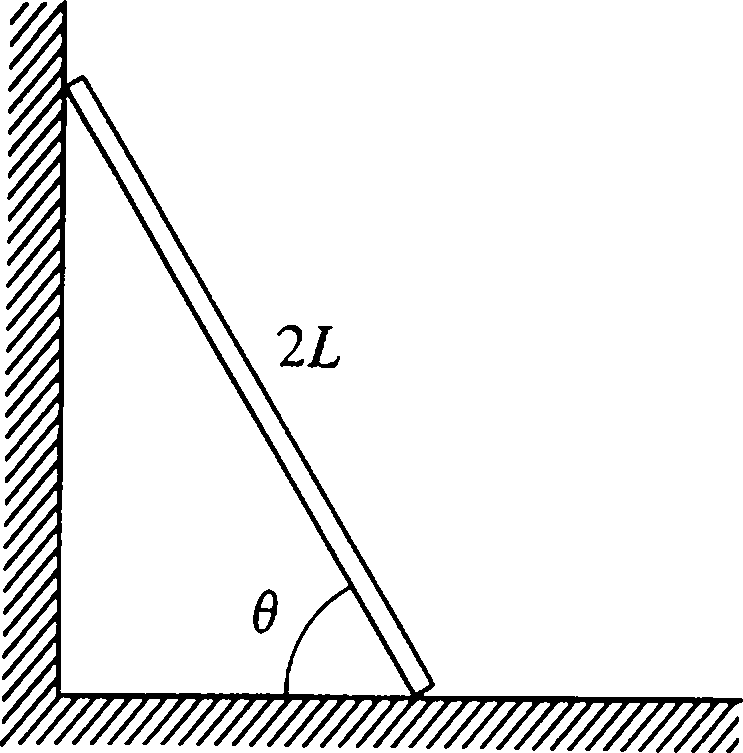
\includegraphics[width=0.25\textwidth]{ps09_7}\end{center}
  \begin{enumerate}[(a)]
    \item Draw a force diagrams showing all the forces acting on the plank. What is the condition that the plank just starts to slip from the wall.
    \item Is the mechanical energy of the plank conserved as it slips down the wall?
    \item What equations arise from the conditions for static equilibrium for both forces and torque? Think about which point to compute the torque about.
    \item Show that the top of the plank loses contact with the wall when it is two-thirds of its initial height against the wall. Hint: only a single variable and its derivatives are needed to describe the motion of the system. Consider the motion of the center of mass of the plank.
  \end{enumerate}
\end{problem}
\begin{solution}
  \begin{enumerate}[(a)]
    \item
  \definecolor{qqwuqq}{rgb}{0,0.39,0}
  \definecolor{zzzzzz}{rgb}{0.6,0.6,0.6}
  \definecolor{zzttqq}{rgb}{0.6,0.2,0}
  \begin{tikzpicture}[line cap=round,line join=round,>=triangle 45,x=1.0cm,y=1.0cm]
  \clip(-1,-1) rectangle (4,5.5);
  \fill[color=zzttqq,fill=zzttqq,fill opacity=0.1] (-3,5.82) -- (0,5.82) -- (0,0) -- (13,0) -- (13,-2.76) -- (-3,-2.76) -- cycle;
  \fill[color=zzzzzz,fill=zzzzzz,fill opacity=0.1] (0,5) -- (0.18,5.11) -- (3.18,0.11) -- (3,0) -- cycle;
  \draw [shift={(3,0)},color=qqwuqq,fill=qqwuqq,fill opacity=0.1] (0,0) -- (120.96:0.6) arc (120.96:180:0.6) -- cycle;
  \draw [color=zzttqq] (-3,5.82)-- (0,5.82);
  \draw [color=zzttqq] (0,5.82)-- (0,0);
  \draw [color=zzttqq] (0,0)-- (13,0);
  \draw [color=zzttqq] (13,0)-- (13,-2.76);
  \draw [color=zzttqq] (13,-2.76)-- (-3,-2.76);
  \draw [color=zzttqq] (-3,-2.76)-- (-3,5.82);
  \draw (0,5)-- (3,0);
  \draw (0,5)-- (0.18,5.11);
  \draw (0.18,5.11)-- (3.18,0.11);
  \draw (3.18,0.11)-- (3,0);
  \draw [->,line width=1.6pt] (1.59,2.55) -- (1.59,0.94);
  \draw [->,line width=1.6pt] (3,0) -- (3,1.61);
  \draw [->,line width=1.6pt] (0,5) -- (1.2,5);
  \draw[color=black] (1.92,2.84) node {$2L$};
  \draw[color=qqwuqq] (2.46,0.46) node {$\theta$};
  \draw[color=black] (1.44,0.94) node {$F_g$};
  \draw[color=black] (3.38,1.76) node {$F_{N,1}$};
  \draw[color=black] (1.68,5.12) node {$F_{N,2}$};
  \end{tikzpicture} \par
  The plank starts to slip when $F_{N,2}$ is 0.
    \item Yes. %\leftturn \rightturn
    \item Let $(x, y)$ be the coordinates of the center of mass.  Then $x = l\cos\theta$ and $y = l\sin\theta$.  Then the equations of linear motion are $$F_{N,2} = m \ddot x$$ and $$F_{N, 1} - m g = m \ddot y.$$ \par
    Since the normal forces do no work, $\frac{1}{2} m v_f^2 + \frac{1}{2} I_{cm} \ddot\theta^2 = -m g \Delta h$, so $$\frac{1}{2} m (\ddot x^2 + \ddot y^2) + \frac{1}{2} I_{cm} \ddot\theta^2  = m g (y_0 - y).$$ \par
    To calculate torque about the center of mass, $\vec \tau = I\vec \alpha = \leftturn F_{N, 1} \cos\theta + \rightturn F_{N, 2}\sin\theta$.  Then $\vec \tau = \leftturn m((\ddot y + g) \cos\theta - \ddot x \sin\theta)$.  Since $I_{cm} = \int_{-l}^l \frac{m}{2l} r^2 \d r = m\frac{l^2}{3}$, $-\left(m\frac{l^2}{3}\right)\ddot\theta = m((\ddot y + g) \cos\theta - \ddot x \sin\theta)$.  Since $F_{N, 2} = 0$, $\ddot x = 0$, so $$-\frac{l^2}{3}\ddot\theta = (\ddot y + g) \cos\theta$$. FIX% Since $x^2 + y^2 = 2l^2$, $$\frac{5}{6}l^2\ddot\theta = \frac{3}{2} x g + y \ddot x - x \ddot y$$ FIX Let $y$ be the height of the vertical contact point and $x$ be the position of the horizontal contact point.  Then, so long as the ladder is in contact with the wall, $x^2 + y^2 = 4 l^2$, that is, since $l$ is constant, $2\dot x + 2\dot y = 0$, and $2\ddot x + 2\ddot y = 0$.  That is, $$\ddot x + \ddot y = 0.$$  Since $y = 2l\sin\theta$ and $x = 2l\cos\theta$, $2l\cos\theta\dot\theta - 2l\sin\theta\dot\theta = 0$, so $\ddot\theta(\cos\theta - \sin\theta) + \dot\theta^2(-\sin\theta -\cos\theta) = 0$, so $$\ddot\theta(\cos\theta - \sin\theta) = \dot\theta^2(\cos\theta + \sin\theta).$$
    %We know that $F_{N, 2} = m \ddot x$ and $m \ddot y = F_{N, 1} - m g$.  Then $\frac{F_{N, 2}}{m} + \frac{F_{N, 1}}{m} - g = 0$, or $$F_{N, 1} + F_{N, 2} = m g.$$  Taking the torque about the center of mass, $\vec \tau = I\vec \alpha = \hat\omega F_{N, 1} x - \hat\omega F_{N,2} y - \hat\omega \frac{x}{2} m g$.  Then $\tau = (m \ddot y - m g) x - m \ddot x y - x m g / 2 = m(x \ddot y - \frac{3}{2} x g - y \ddot x)$.  Since $I = m d^2 + \int_{-l}^l \frac{m}{2l} r^2 \d r = \frac{m}{2l} \frac{x^2 + y^2}{4} + m \frac{2 l^3}{3}$, $-\left(m \frac{x^2 + y^2}{4} + \frac{l^2}{3}\right)\ddot\theta = m(x \ddot y - \frac{3}{2} x g - y \ddot x)$.  Since $x^2 + y^2 = 2l^2$, $$\frac{5}{6}l^2\ddot\theta = \frac{3}{2} x g + y \ddot x - x \ddot y$$ %Taking the torque about the lower left corner, $\vec \tau = I\vec \alpha = \hat\omega F_{N, 1} x - \hat\omega F_{N,2} y - \hat\omega \frac{x}{2} m g$.  Then $\tau = (m \ddot y - m g) x - m \ddot x y - x m g / 2 = m(x \ddot y - \frac{3}{2} x g - y \ddot x)$.  Since $I = m d^2 + \int_{-l}^l \frac{m}{2l} r^2 \d r = \frac{m}{2l} \frac{x^2 + y^2}{4} + m \frac{2 l^3}{3}$, $-\left(m \frac{x^2 + y^2}{4} + \frac{l^2}{3}\right)\ddot\theta = m(x \ddot y - \frac{3}{2} x g - y \ddot x)$.  Since $x^2 + y^2 = 2l^2$, $$\frac{5}{6}l^2\ddot\theta = \frac{3}{2} x g + y \ddot x - x \ddot y$$.

      The point at which the horizontal contact force is zero requires that $\ddot x = 0$.  Then     FIX What equations arise from the conditions for static equilibrium for both forces and torque? Think about which point to compute the torque about.
    \item FIX Show that the top of the plank loses contact with the wall when it is two-thirds of its initial height against the wall. Hint: only a single variable and its derivatives are needed to describe the motion of the system. Consider the motion of the center of mass of the plank.
  \end{enumerate}
\end{solution}


\end{document}
